\begin{figure*}
\centering
%\vspace*{-0.3cm}  
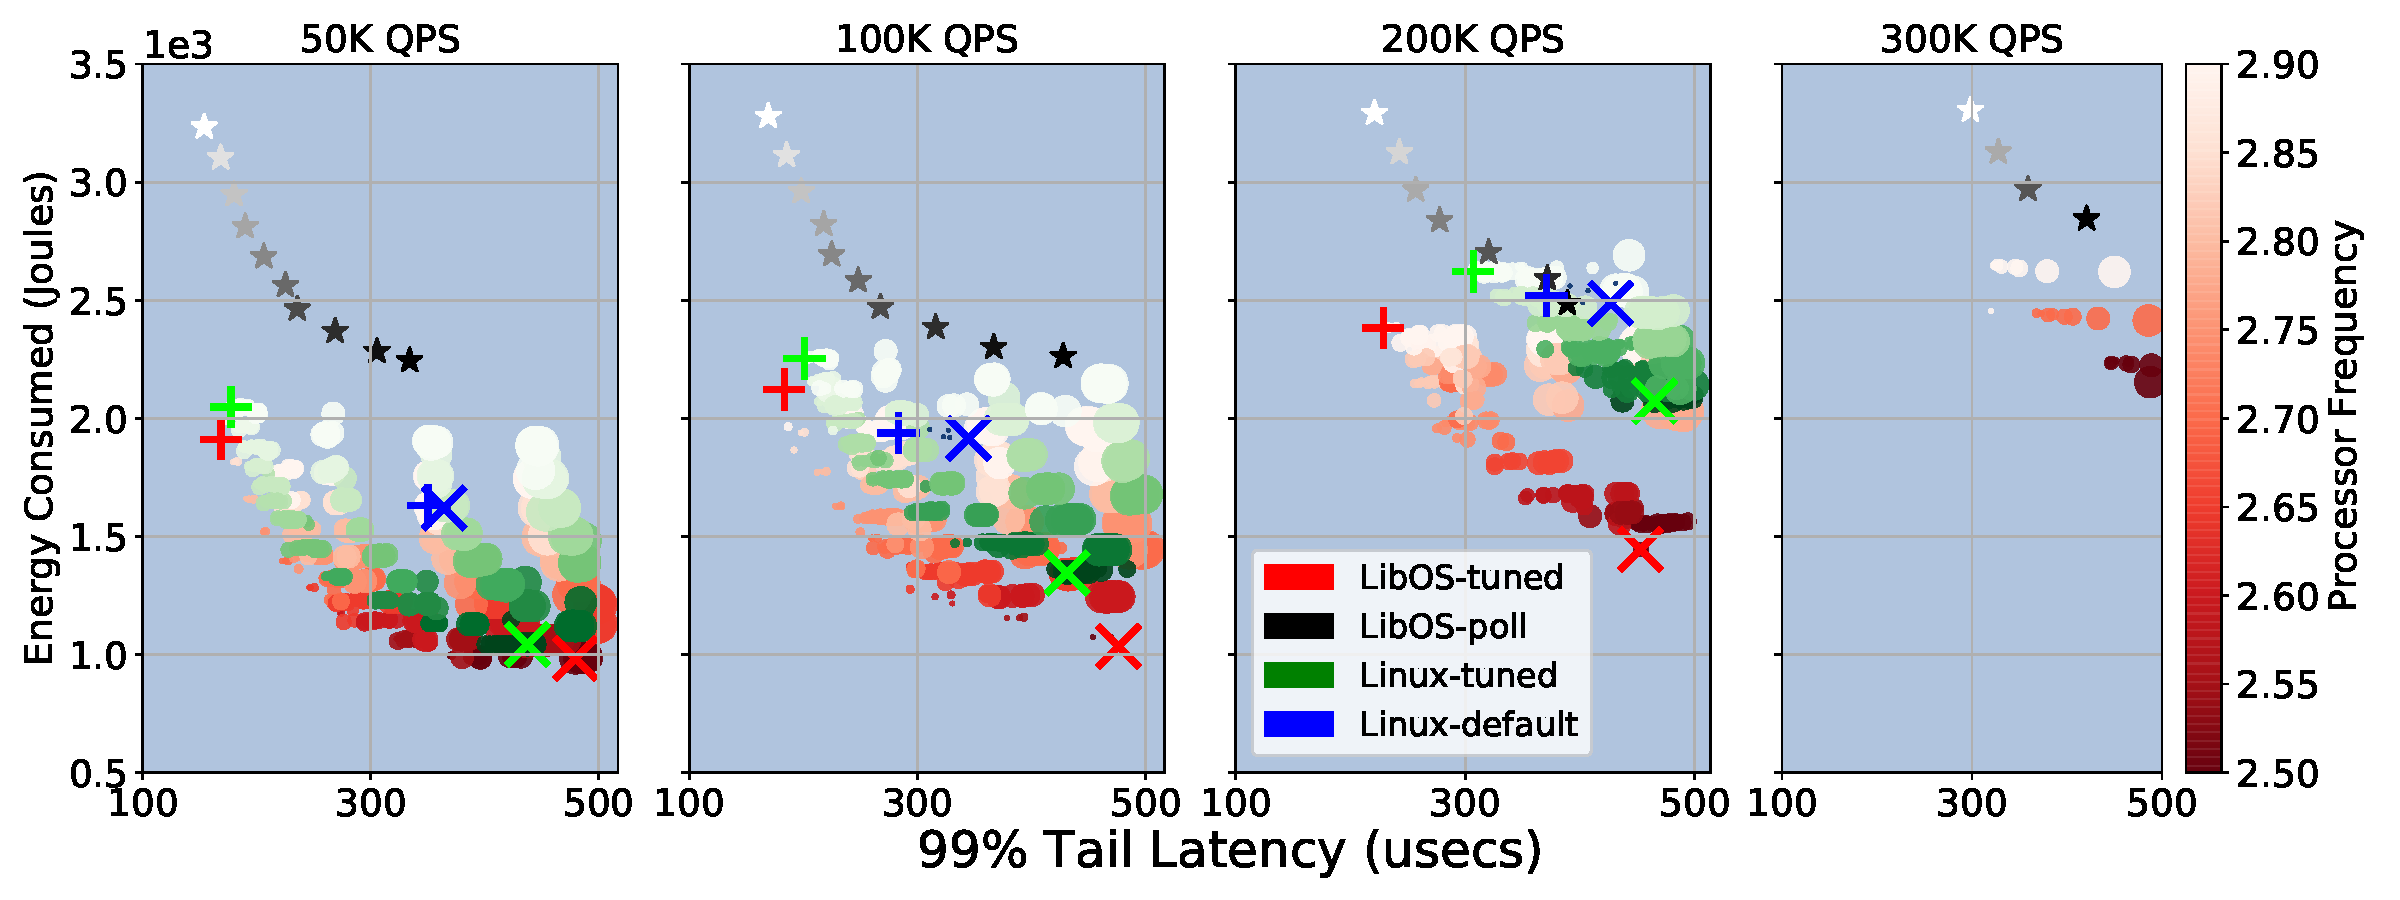
\includegraphics[width=1\textwidth]{figures/mcdsilo_overview}
\vspace*{-8mm}
\caption[]
%{\small 
{Overview of memcached-silo experiments across 50K, 100K, 200Km and 300K QPS. The larger the size of a point equates to slower interrupt delay. The darkening of color gradient indicates slowing down processor more. The \textbf{x} indicate lowest energy consumption. The \textbf{+} indicate lowest tail latency.}
\label{fig:mcdsilo_overview}
\end{figure*}

\begin{figure}
%\centering
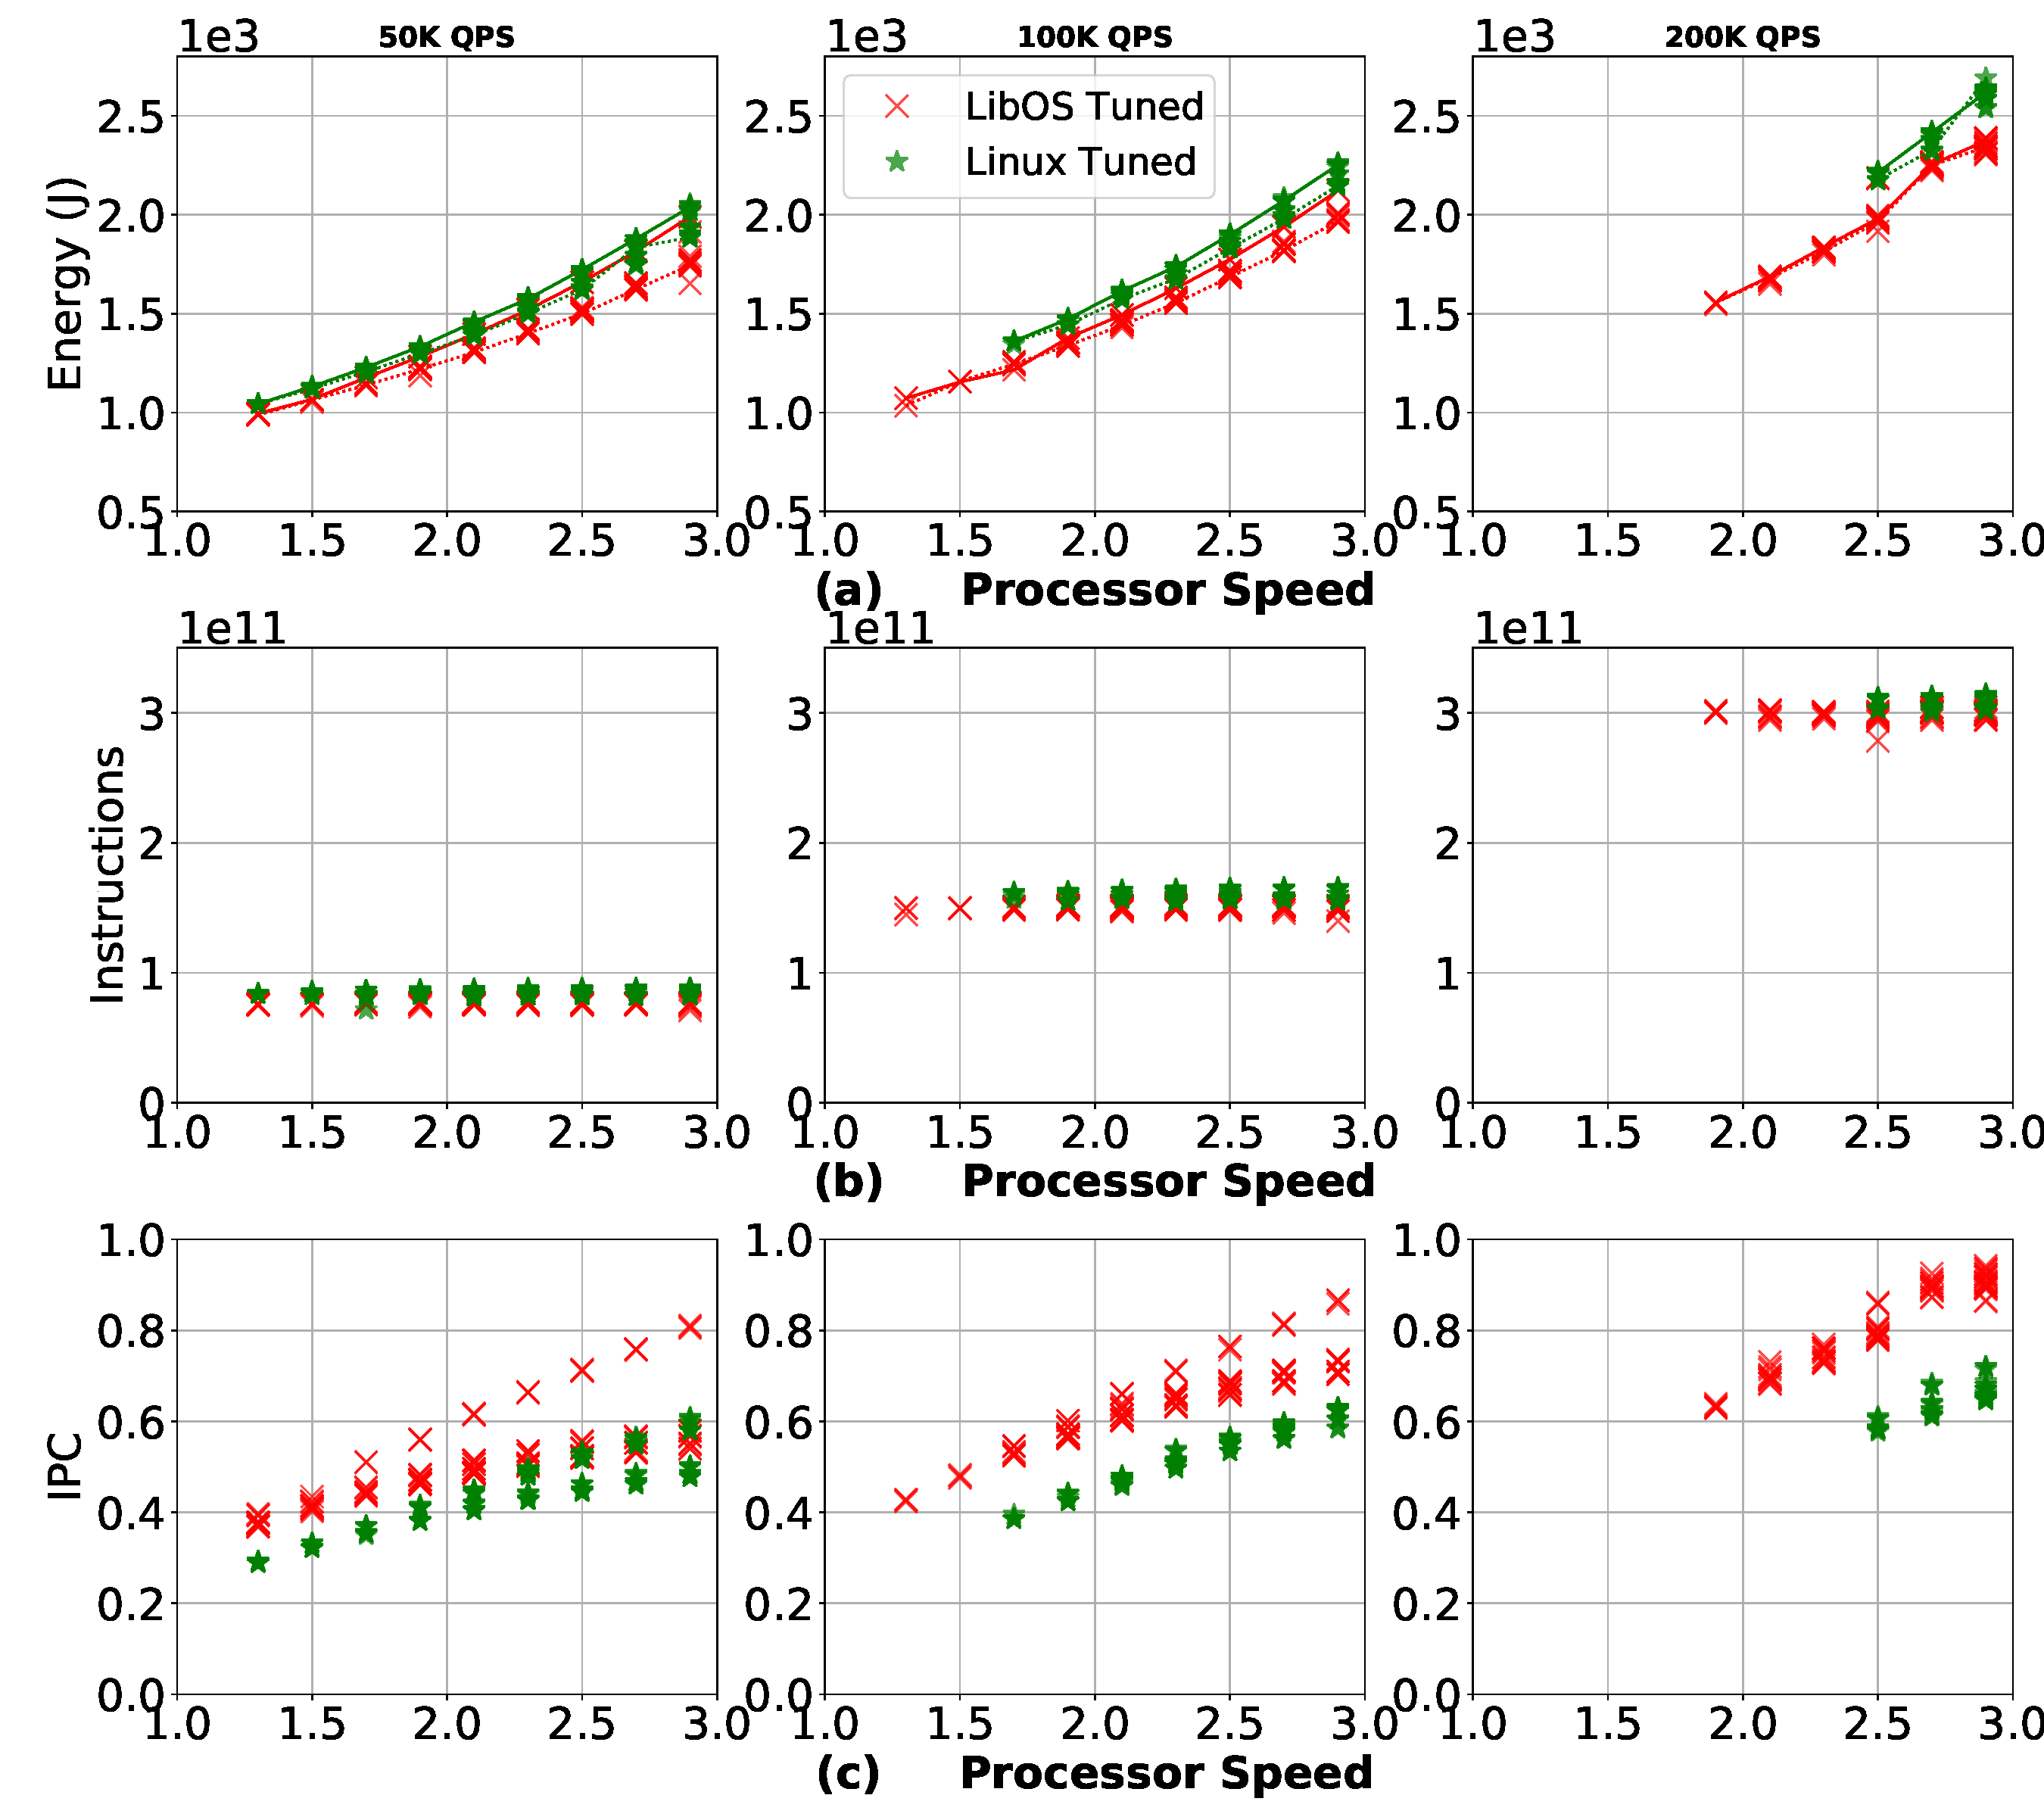
\includegraphics[width=0.5\textwidth]{figures/mcdsilo_detail}
%\hspace*{-10.0cm} 
%\vspace*{-1.0cm}  
\vspace*{-8mm}
\caption[]{Detailed plots of some gathered statistics of the above QPS loads. Compares LibOS-tuned and Linux-tuned.}
\label{fig:mcdsilo_detail}
%\vspace*{-.25in}
\end{figure}

\subsection{Memcached-silo}
\label{sec:mcdsilo}
Memcached-silo is a open loop workload built on top of the normal memcached protocol. It is computationally and memory more intensive than regular memcached as it incorporates both latency-sensitive network compute and memory-intensive TPC-C style transaction processing. The workload is structured such that on every memcached request, it triggers a corresponding set of TPC-C transaction processing logic on a in-memory database~\cite{silo}. We ported the memcached-silo implementation~\cite{mcdsilo, zygos} to our library OS interfaces. The workload mix and SLA constraints of memcached-silo follow from those used in the memcached experiments in \cref{sec:mcd}. Given its application heavier nature, we only needed two 16-core client nodes at 16 connections per core to saturate a single 16-core memcached-silo server. 

\subsubsection{Slowing down has benefits even in computationally heavy workloads}
\label{sec:mcdsilo:dvfstradeoff}
In contrast to figure~\ref{fig:mcd_overview}, figure~\ref{fig:mcdsilo_overview} illustrates that as application becomes larger in each memcached request; the trade-offs of tail latency and energy become discernible in both Linux and the library OS (color gradient darkens in horizontal manner). Even in a computation heavy workload under a stringent SLA, it is still possible to use delay both processor and interrupts to further save energy (shown in figure~\ref{fig:mcdsilo_detail}(a)). Similar to figure~\ref{fig:mcd_detail_1}(a), figure~\ref{fig:mcdsilo_detail}(a) shows that slowing the processor results in the most energy savings and using interrupt delays on top leads to additional savings. However, in contrast to figure~\ref{fig:mcd_detail_1}(a), the effects of delayed interrupts is greatly diminished as the QPS load increases. One can also see this effect in the 100K and 200K QPS where the configuration that yielded Min-Energy for the library OS uses a small dot. This observation harkens back to the implications of a slowed processor on the packet processing path (\cref{sec:workflow:dvfs}); furthermore, this effect is exacerbated as application logic is heavier.

\subsubsection{Library OS IPC efficiency surprises}
\label{sec:mcdsilo:ipc}
Even though figure~\ref{fig:mcdsilo_detail}(a) demonstrate similar number of instructions between Linux and the library OS, the IPC measurement in figure~\ref{fig:mcdsilo_detail}(c) reveals a specialized OS can execute instructions more efficiently even in a application bound workload. This IPC benefit not only leads to energy efficiency but also creates more slack for the library OS to take advantage of slow down. Figure~\ref{fig:mcdsilo_detail}(a) shows that at faster processor speeds in the 50K and 100K QPS, the library OS was still able to slow down interrupt delays to save more energy than Linux by 50\% even in computationally heavy workload.

%\subsubsection{Finding-1: Implications of OS path length efficiency}

% ebbrt_tuned c1 4 0x1d00 135    159.0 1954.58
% ebbrt_tuned c1e 4 0x1d00 135   203.1 1789.93
% ebbrt_tuned c3 4 0x1d00 135    205.2 1779.41
% ebbrt_tuned c7 4 0x1d00 135    206.0 1789.72
% ebbrt_tuned c1 200 0xd00 135   471.5 991.89
% ebbrt_tuned c1e 200 0xd00 135  483.5 990.82
% ebbrt_tuned c3 200 0xd00 135   488.0 987.11
% ebbrt_tuned c7 200 0xd00 135   488.4 989.57

% ebbrt_tuned c1 2 0x1d00 135 304.2 2631.54
% ebbrt_tuned c1e 2 0x1d00 135 312.0 2637.85
% ebbrt_tuned c3 2 0x1d00 135 322.5 2631.96
% ebbrt_tuned c7 2 0x1d00 135 326.9 2646.27

% ebbrt_tuned c1 100 0x1900 135 481.8 2210.25
% ebbrt_tuned c1e 100 0x1900 135 486.1 2051.88
% ebbrt_tuned c3 100 0x1900 135 491.8 2209.09
% ebbrt_tuned c7 100 0x1900 135 492.4 2214.79

% \begin{table}[t]
% \centering
% \begin{tabular}{l|c|c|c|c|c|}
%   QPS & Type & Sleep State & Latency (\SI{}{\micro s}) & Energy (\SI{}{\joule})\\ \hline
%   50K & Min-Tail & C1 & 159 & 1954\\ \hline
%   50K & Min-Tail & C1E & 203 & 1789\\ \hline
%   50K & Min-Tail & C3 & 205 & 1779\\ \hline
%   50K & Min-Tail & C7 & 206 & 1789\\ \hline
%   50K & Min-Energy & C1 & 471 & 991\\ \hline
%   50K & Min-Energy & C1E & 483 & 990\\ \hline
%   50K & Min-Energy & C3 & 488 & 987\\ \hline
%   50K & Min-Energy & C7 & 488 & 989\\ \hline
%   300K & Min-Tail & C1 & 304 & 2631\\ \hline
%   300K & Min-Tail & C1E & 312 & 2637\\ \hline
%   300K & Min-Tail & C3 & 322 & 2631\\ \hline
%   300K & Min-Tail & C7 & 326 & 2646\\ \hline
%   300K & Min-Energy & C1 & 481 & 2210\\ \hline
%   300K & Min-Energy & C1E & 486 & 2207\\ \hline
%   300K & Min-Energy & C3 & 491 & 2209\\ \hline
%   300K & Min-Energy & C7 & 492 & 2214\\ \hline
% \end{tabular}
% \caption{Min-Tail refers to configuration of processor speed and interrupt rate where the lowest tail latency was achieved and Min-Energy refers to the configuration with lowest energy use.}
% %\caption{Workload configurations.
% %The column {\em Nature} indicates open-versus-closed loop nature
% %and {\em CPU} indicates application CPU demand.}
% \label{table:mcdsilo_sleep_states}	
% \end{table}
%\subsubsection{Finding-1: Implications of OS path length efficiency}
